%%%%%%%%%%%%%%%%%%%%%%%%%%%%%%%%%%%%%%%%%%%%%%%%%%%%%%%%%%%%%%%%%%%%%%%%%%%%%%%%
%2345678901234567890123456789012345678901234567890123456789012345678901234567890
%        1         2         3         4         5         6         7         8

\documentclass[letterpaper, 10 pt, conference]{ieeeconf}  % Comment this line out
                                                          % if you need a4paper
%\documentclass[a4paper, 10pt, conference]{ieeeconf}      % Use this line for a4
                                                          % paper

\IEEEoverridecommandlockouts%                             % This command is only
                                                          % needed if you want to
                                                          % use the \thanks command
\overrideIEEEmargins%
% See the \addtolength command later in the file to balance the column lengths
% on the last page of the document

\usepackage[utf8]{inputenc}
\usepackage[T1]{fontenc}
\usepackage{url}
\usepackage{graphicx}
\usepackage{float}
\urlstyle{same}

% The following packages can be found on http:\\www.ctan.org
%\usepackage{graphics} % for pdf, bitmapped graphics files
%\usepackage{epsfig} % for postscript graphics files
%\usepackage{mathptmx} % assumes new font selection scheme installed
%\usepackage{mathptmx} % assumes new font selection scheme installed
%\usepackage{amsmath} % assumes amsmath package installed
%\usepackage{amssymb}  % assumes amsmath package installed

\title{\LARGE \bf
Learning Expressive Humanoid Locomotion from Monocular Runway Videos
}

%\author{ \parbox{3 in}{\centering Huibert Kwakernaak*
%         \thanks{*Use the $\backslash$thanks command to put information here}\\
%         Faculty of Electrical Engineering, Mathematics and Computer Science\\
%         University of Twente\\
%         7500 AE Enschede, The Netherlands\\
%         {\tt\small h.kwakernaak@autsubmit.com}}
%         \hspace*{ 0.5 in}
%         \parbox{3 in}{ \centering Pradeep Misra**
%         \thanks{**The footnote marks may be inserted manually}\\
%        Department of Electrical Engineering \\
%         Wright State University\\
%         Dayton, OH 45435, USA\\
%         {\tt\small pmisra@cs.wright.edu}}
%}

\author{}


\begin{document}



\maketitle
\thispagestyle{empty}
\pagestyle{empty}


%%%%%%%%%%%%%%%%%%%%%%%%%%%%%%%%%%%%%%%%%%%%%%%%%%%%%%%%%%%%%%%%%%%%%%%%%%%%%%%%
\begin{abstract}

Runway walking uses posture, stride, and foot placement to present clothing and express a particular style. However, humanoid robots in fashion shows usually use walking policies designed mainly for balance and speed. We present an end-to-end pipeline that converts a monocular runway video into a deployable humanoid policy through motion recovery, robot retargeting, motion correction, policy training, simulation testing, and physical deployment. We evaluate the pipeline on the Booster K1 using a runway-style motion. The learned policy completed all 20 physical trials without falling and reproduced narrow foot placement together with coordinated leg, torso, and arm movements. Its measured step width ranged from $-0.8$ to 1.8 cm, compared with 5.1 to 11.4 cm for the standard K1 walk, and included occasional crossover steps.


\end{abstract}


%%%%%%%%%%%%%%%%%%%%%%%%%%%%%%%%%%%%%%%%%%%%%%%%%%%%%%%%%%%%%%%%%%%%%%%%%%%%%%%%
\section{INTRODUCTION}

% Catwalking is a distinct, context-conditioned, garment-mediated form of expressive locomotion. Its purpose is not merely to move a body from one end of a runway to another, but to present clothing, communicate a show’s aesthetic, coordinate with choreography, and produce a legible performance for an audience and cameras. A conventional humanoid gait primarily solves transport: follow a velocity command, remain upright, minimize energy, and recover from disturbances. A catwalk must solve all of those problems while also controlling how the body and therefore the garment is perceived.

The catwalk is a specialized form of expressive locomotion in which posture, cadence, stride, foot placement, arm motion, gaze, posing, and turning are coordinated to present a garment and communicate the aesthetic of a fashion show. Unlike ordinary walking, its objective is not only stable movement, but also the control of silhouette, drape, rhythm, and perceived character. Catwalk styles vary across designers, garments, footwear, and show direction, making runway walking a context-dependent performance rather than a single fixed gait.

Humanoid robots used in fashion shows typically rely on conventional locomotion policies optimized for balance, velocity tracking, and disturbance recovery. While these policies allow robots to traverse a runway, they do not address the expressive or garment-presentation functions of the catwalk. Prior work has examined expressive robot gait and isolated fashion-model-like motion, but there remains no general data-driven framework for learning multiple runway styles from human demonstrations and transferring them to physical humanoids. We therefore formulate robotic catwalking as a style-conditioned locomotion problem evaluated through both quantitative measures of motion and stability and qualitative judgments of style, confidence, and fashion-show appropriateness.

% Humanoid robots are becoming better at walking, but most systems still focus mainly on stability and speed. In areas such as fashion, entertainment, and public demonstrations, the style of the motion can be just as important. A robot may need to reproduce a specific walk or performance rather than use a standard gait.

Video is a simple way to provide such a motion. Instead of manually creating robot trajectories, the user can show the desired behavior in a monocular video. The main difficulty is that motion recovery, retargeting, training, and deployment are usually handled by separate tools with different formats and configurations.

In this work, we present an end-to-end pipeline that takes a human video and produces a policy ready to run on a humanoid robot. The user provides the video and selects the target robot, while the pipeline handles motion recovery, retargeting, correction, training, simulation testing, and deployment.

We demonstrate the pipeline on the Booster K1 using runway-style catwalk motion. Catwalk walking is our main example, but the same workflow can be used for other custom motions in fashion, entertainment, and related applications.



%%%%%%%%%%%%%%%%%%%%%%%%%%%%%%%%%%%%%%%%%%%%%%%%%%%%%%%%%%%%%%%%%%%%%%%%%%%%%%%%
\section{RELATED WORK}

Gravity-View Human Motion Recovery (GVHMR)~\cite{gvhmr} converts a video into 3D human motion aligned with the ground. General Motion Retargeting (GMR)~\cite{gmr} then adapts the motion to the selected robot.

BeyondMimic~\cite{beyondmimic} uses the retargeted motion to train a tracking policy in the Booster training framework~\cite{boostertrain}. The policy is tested and run on the robot with the Booster deployment framework~\cite{boosterdeploy}. These frameworks cover separate stages of the process but do not provide a single workflow from video to robot.

Previous work has explored fashion-inspired and expressive robot walking. Or~\cite{fashionmodelrobot} simulated fashion-model-like motions on a humanoid, while Huzaifa et al.~\cite{expressivegait} generated and evaluated different expressive gaits. Kobayashi et al.~\cite{catwalkstyles} identified leg crossing as a difference among runway styles, motivating our use of step width to compare the learned policy with the standard K1 walk.



%%%%%%%%%%%%%%%%%%%%%%%%%%%%%%%%%%%%%%%%%%%%%%%%%%%%%%%%%%%%%%%%%%%%%%%%%%%%%%%%


\section{METHOD}

Our pipeline turns a monocular video of human motion into a policy that can be tested and run on a humanoid robot. The user provides the video and selects a robot supported by GMR~\cite{gmr}. The pipeline handles 3D motion generation, retargeting, motion correction, policy training, and deployment.

\begin{figure}[H]
    \centering
    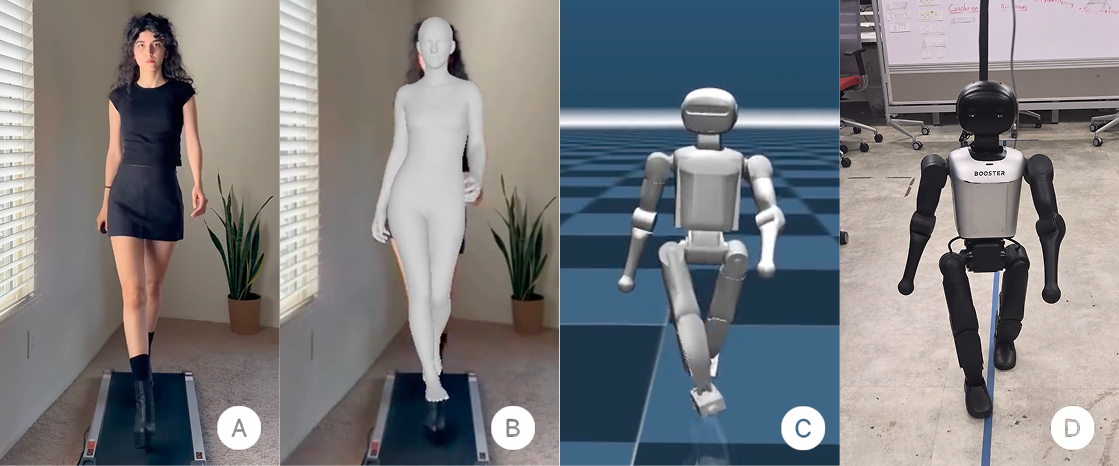
\includegraphics[width=\columnwidth]{pipeline_strip.png}
    \caption{Overview of the pipeline: (a) monocular runway video, (b) recovered 3D human motion, (c) retargeted robot motion in simulation, and (d) physical deployment on the Booster K1.}
    \label{fig:pipeline_strip}
\end{figure}

\subsection{Motion Recovery}

The pipeline uses GVHMR~\cite{gvhmr} to convert the input video into 3D human motion. It reads the video's frame rate and selects the setting for a static or moving camera. The resulting SMPL-X motion and global path are then sent to the retargeting stage.

\subsection{Robot Retargeting}

The user selects a robot supported by GMR~\cite{gmr}. GMR adapts the human motion to the robot's body proportions and joints. The output is a motion trajectory for the selected robot.

\subsection{Motion Correction and Conversion}

After retargeting, the pipeline detects foot contacts and adjusts the motion to keep the feet aligned with the floor. It also removes vertical drift without changing the joint angles, which helps preserve the original walking style. Finally, the motion is converted into the training format with the robot joint states, base pose, and frame timing from the source video.

\subsection{Policy Training}

The processed motion is used as the reference trajectory for training with BeyondMimic~\cite{beyondmimic} in the Booster training framework~\cite{boostertrain}. We use the existing training method while keeping the actuator limits, stiffness, damping, and action scaling consistent with the deployment configuration. This avoids using a policy on hardware with different control settings from those used during training.

\subsection{Simulation and Deployment}

After training, the exported policy is loaded into the Booster deployment framework~\cite{boosterdeploy} and tested in MuJoCo using the deployment controller. This sim-to-sim test is used to check balance, tracking, and joint behavior before hardware execution. The same exported policy can then be launched on the physical robot with our deployment script. The final output of the workflow is therefore a runnable robot policy rather than only a retargeted trajectory or training checkpoint.

%%%%%%%%%%%%%%%%%%%%%%%%%%%%%%%%%%%%%%%%%%%%%%%%%%%%%%%%%%%%%%%%%%%%%%%%%%%%%%%%
\section{EXPERIMENTAL SETUP}

The catwalk policy was trained using BeyondMimic in the Booster training framework and first tested in MuJoCo. The trained policy was then deployed on the Booster K1 through a custom deployment script and a wired Ethernet connection.

A straight 5 m walking path was marked on the floor using tape. The markings indicated the starting position, runway centerline,and distance intervals used to measure the traveled distance and step width. Each test contained approximately 23 steps. Safety belts were attached to the robot to prevent damage in the event of a fall while remaining loose during normal walking.

%%%%%%%%%%%%%%%%%%%%%%%%%%%%%%%%%%%%%%%%%%%%%%%%%%%%%%%%%%%%%%%%%%%%%%%%%%%%%%%%
\section{RESULTS}

\subsection{Physical Execution}

The learned policy completed all 20 physical trials without falling, with approximately 23 steps in each trial. The robot showed narrow foot placement and coordinated leg, torso, and arm movements. The first step sometimes caused a small lateral offset, after which the robot continued along a stable path approximately parallel to the runway line.

\subsection{Foot-Placement Comparison}

We compared the lateral distance between consecutive foot placements using 12 steps from the standard K1 walk and 23 steps from the learned catwalk policy. Negative values indicate crossover steps, where one foot was placed beyond the other foot laterally.

The standard K1 walk produced step widths between 5.1 and 11.4 cm, while the catwalk policy produced widths between $-0.8$ and 1.8 cm These results show that the learned policy produced substantially narrower foot placement and occasional crossover steps compared with the standard K1 walk.

%%%%%%%%%%%%%%%%%%%%%%%%%%%%%%%%%%%%%%%%%%%%%%%%%%%%%%%%%%%%%%%%%%%%%%%%%%%%%%%%
\section{FUTURE WORK}

Future work includes developing a controllable policy, creating a larger catwalk motion dataset, improving the evaluation metrics and involving fashion experts in assessment of the robot's walking style and training and deploying the pipeline on humanoid robots beyond the Booster K1.


%%%%%%%%%%%%%%%%%%%%%%%%%%%%%%%%%%%%%%%%%%%%%%%%%%%%%%%%%%%%%%%%%%%%%%%%%%%%%%%%

\begin{thebibliography}{99}

\bibitem{gvhmr} Z. Shen, H. Pi, Y. Xia, Z. Cen, S. Peng, Z. Hu, H. Bao, R. Hu, and X. Zhou, ``World-grounded human motion recovery via gravity-view coordinates,'' in \emph{Proc. SIGGRAPH Asia 2024 Conf. Papers}, Tokyo, Japan, 2024, Art. no. 144, pp. 1--11, doi: 10.1145/3680528.3687565.

\bibitem{gmr} J. P. Ara\'{u}jo, Y. Ze, P. Xu, J. Wu, and C. K. Liu, ``Retargeting matters: General motion retargeting for humanoid motion tracking,'' \emph{arXiv preprint arXiv:2510.02252}, 2025, doi: 10.48550/arXiv.2510.02252.

\bibitem{beyondmimic} T. E. Truong, Q. Liao, X. Huang, G. Tevet, C. K. Liu, and K. Sreenath, ``BeyondMimic: From motion tracking to versatile humanoid control via guided diffusion,'' \emph{arXiv preprint arXiv:2508.08241}, 2025, doi: 10.48550/arXiv.2508.08241.

\bibitem{boostertrain} Booster Robotics, \emph{booster\_train}, GitHub repository. [Online]. Available: \url{https://github.com/BoosterRobotics/booster_train}. Accessed: Aug. 5, 2026.

\bibitem{boosterdeploy} Booster Robotics, \emph{booster\_deploy}, GitHub repository. [Online]. Available: \url{https://github.com/BoosterRobotics/booster_deploy}. Accessed: Aug. 5, 2026.

\bibitem{catwalkstyles} Y. Kobayashi, S. Saito, and T. Murahori, ``Classification of fashion models' walking styles using publicly available data, pose detection technology, and multivariate analysis: From past to current trendy walking styles,'' \emph{Sensors}, vol. 24, no. 12, Art. no. 3865, 2024, doi: 10.3390/s24123865.

\bibitem{fashionmodelrobot} J. Or, ``Computer simulations of a humanoid robot capable of walking like fashion models,'' \emph{IEEE Trans. Syst., Man, Cybern. C, Appl. Rev.}, vol. 42, no. 2, pp. 241--248, Mar. 2012, doi: 10.1109/TSMCC.2011.2115238.

\bibitem{expressivegait} U. Huzaifa, C. Maguire, and A. LaViers, ``Toward an expressive bipedal robot: Variable gait synthesis and validation in a planar model,'' \emph{Int. J. Social Robot.}, vol. 12, no. 1, pp. 129--141, Jan. 2020, doi: 10.1007/s12369-019-00547-6.

\end{thebibliography}

\end{document}
